% This is samplepaper.tex, a sample chapter demonstrating the
% LLNCS macro package for Springer Computer Science proceedings;
% Version 2.20 of 2017/10/04
%
\documentclass[runningheads]{llncs}
%
\usepackage{graphicx}
\usepackage{amsmath,mathtools,listings,inconsolata,booktabs}
% Used for displaying a sample figure. If possible, figure files should
% be included in EPS format.
%
% If you use the hyperref package, please uncomment the following line
% to display URLs in blue roman font according to Springer's eBook style:
% \renewcommand\UrlFont{\color{blue}\rmfamily}

\graphicspath{{.}{./images/}}

\newcommand*{\cc}[2]{\multicolumn{1}{#1}{#2}}
\newcommand*{\ttd}[1]{\texttt{\detokenize{#1}}}
\newcommand*{\sld}[1]{\textsl{\detokenize{#1}}}

\begin{document}
%
\title{Doors}
%
%\titlerunning{Abbreviated paper title}
% If the paper title is too long for the running head, you can set
% an abbreviated paper title here
%
\author{Bruno Carvalho up201606517 \and Amadeu Pereira up201605646}
%
%\authorrunning{F. Author et al.}
% First names are abbreviated in the running head.
% If there are more than two authors, 'et al.' is used.
%
\institute{Faculdade de Engenharia da Universidade do Porto}		%\email{\{abc,lncs\}@uni-heidelberg.de}

\maketitle

\begin{abstract}
In this paper we describe and explore a simple restraint logic programming solution for the logic problem \textit{Doors}.

\keywords{doors \and logic puzzle \and rooms}
\end{abstract}

\section{Problem Description}
\label{sec:description}

The logic problem \textit{Doors} is a puzzle on a rectangular board whose cells are either empty or contain natural numbers. The board is thought of like a \textit{house}. Each cell is a \textit{room}, and two adjacent cells are separated by a \textit{wall} with one \textit{door}. That door may be either open or closed. If it is open, then the cell can \textsl{see} its adjacent room through the doorway. A man standing in a room can look in all four directions --- north, east, west, south --- and count the number of \textit{visible rooms}.

The puzzle consists in discovering an assignment of open and closed doors to the walls of the board such that the natural number in each non-empty cell is how many rooms are visible from that cell (including itself). There may be multiple solutions, or none at all.

\subsection{Examples}

\begin{equation*}
\arraycolsep=4.0pt\def\arraystretch{1.3}
\begin{array}[c]{|c c c c|}
\hline
4 & \cc{ c|}{2} & \cc{|c }{4} & 2\\
\cline{2-2}\cline{4-4}
5 & \cc{ c }{3} & \cc{ c|}{5} & 3\\
\cline{2-2}
4 & \cc{ c|}{3} & \cc{|c }{ } & 4\\
\cline{1-1}\cline{3-3}
2 & \cc{ c|}{3} & \cc{|c }{2} & 4\\
\hline
\end{array}
\qquad
\begin{array}[c]{|c c c c c c|}
\hline
3 & \cc{ c|}{5} & \cc{|c }{3} & \cc{ c|}{2} & \cc{|c }{2} & 5\\
\cline{4-5}
  & \cc{|c|}{ } & \cc{|c }{4} & \cc{ c }{5} & \cc{ c|}{ } &  \\
\cline{1-1}\cline{3-3}\cline{5-5}
4 & \cc{ c }{6} & \cc{ c|}{4} & \cc{|c }{5} & \cc{ c }{ } & 6\\
\cline{5-5}
5 & \cc{ c }{7} & \cc{ c }{5} & \cc{ c|}{6} & \cc{|c|}{1} & 4\\
\hline
\end{array}
\qquad
\begin{array}[c]{|c c c c c c|}
\hline
2 & \cc{|c|}{1} & \cc{|c|}{4} & \cc{|c|}{ } & \cc{|c|}{ } & 1\\
\cline{2-2}\cline{4-4}\cline{6-6}
2 & \cc{|c }{2} & \cc{ c|}{5} & \cc{|c }{5} & \cc{ c }{6} & 4\\
\cline{1-2}
1 & \cc{|c }{3} & \cc{ c|}{5} & \cc{|c }{4} & \cc{ c|}{5} & 2\\
\cline{1-1}\cline{6-6}
  & \cc{|c }{3} & \cc{ c|}{5} & \cc{|c }{5} & \cc{ c }{6} & 3\\
\hline
\end{array}
\end{equation*}

\section{Approach}
\label{sec:approach}

A puzzle of size $n\times m$ is represented internally by three matrices (list of lists): \textsl{Board}, of size $n\times m$, holding the cell numbers; \textsl{Vertical}, of size $n\times (m-1)$, holding the vertical walls; and \textsl{Horizontal}, of size $(n-1)\times m$, holding the horizontal walls.

For each cell $(R,C), R=1,2,\cdots,n, C=1,2,\cdots,m$, indices in \textsl{Board}, the left wall has index $(R,C-1)$ in \textsl{Vertical}, the right wall has index $(R,C)$ in \textsl{Vertical}, the top wall has index $(R-1,C)$ in \textsl{Horizontal}, the bottom wall has index $(R,C)$ in \textsl{Horizontal}.
Each wall in the board is assigned the number 0 for closed door and 1 for open door.

\subsection{Restrictions}
\label{subsec:solutionrestrictions}

When solving a puzzle \textsl{Board} is fully instantiated, while \textsl{Vertical} and \textsl{Horizontal} contain domain variables (domain $\{0,1\}$). Empty cells in the \textsl{Board} are represented by a $0$, as it is never a valid visible room counter.

\begin{equation*}
\arraycolsep=4.0pt\def\arraystretch{1.3}
\begin{array}[c]{|c c c c c c c c|}
\hline
1 & \cc{ c }{T} & \cc{ c }{?} & \cc{ c }{?} & \cc{ c }{?} & \cc{ c }{?} & \cc{ c }{?} & 2\\
%
X & \cc{ c }{A} & \cc{ c }{B} & \cc{ c }{C} & \cc{ c }{D} & \cc{ c }{E} & \cc{ c }{F} & G\\
%
? & \cc{ c }{M} & \cc{ c }{?} & \cc{ c }{?} & \cc{ c }{?} & \cc{ c }{?} & \cc{ c }{?} & ?\\
%
? & \cc{ c }{N} & \cc{ c }{?} & \cc{ c }{?} & \cc{ c }{?} & \cc{ c }{?} & \cc{ c }{?} & ?\\
\hline
\end{array}
\end{equation*}

Consider the puzzle above. The horizontal range $A-G$ consists of $7$ rooms and $6$ vertical doors: let $\{b,c,d,e,f,g\}$ be these vertical doors, from left to right.

Focus on room $A$.
If $b=0$ then $A$ sees no rooms to its right. If $b=1$ and $c=0$ then $A$ sees only room $B$.
A general formula can be deduced by noticing that closed doors behave as zero elements.

Let $e_A$ be the total number of rooms $A$ sees to its right (east), then

\begin{equation}\label{eq:acc}
e_A=b+b(c+c(d+d(e+e(f+f(g+g\cdot 0)))))
\end{equation}

Now, if we analogously define $w_A$ for west, $n_A$ for north and $s_A$ for south, then we find that the number in cell $A$ must be $e_A+w_A+n_A+s_A+1$.

Implementing these restrictions in \texttt{PROLOG} is surprisingly simple. We start with a predicate to compute formula:

\begin{center}
\begin{minipage}{0.45\textwidth}
\centering\ttfamily
\begin{lstlisting}[language=Prolog]
calculate_value([], 0).
calculate_value([H|T], V) :-
    calculate_value(T, V1),
    V #= H + H*V1.
\end{lstlisting}
\end{minipage}
\end{center}

Then, for each non-zero cell $(R,C)$ on the \textsl{Board}, we retrieve as a list the four ranges of doors to the right, left, top and bottom of $(R,C)$, apply the formula for each list, and finally the restriction:

\begin{center}
\begin{minipage}{0.85\textwidth}
\centering\ttfamily
\begin{lstlisting}[language=Prolog]
restrict_cell(Board, _, _, [R,C]) :-
    matrixnth1([R,C], Board, 0), !. % empty cell
restrict_cell(Board, Vertical, Horizontal, [R,C]) :-
    matrixnth1([R,C], Board, Value),
    right_total(Vertical, [R,C], Right),
    left_total(Vertical, [R,C], Left),
    top_total(Horizontal, [R,C], Top),
    bot_total(Horizontal, [R,C], Bot),
    Right + Left + Top + Bot + 1 #= Value.
\end{lstlisting}
\end{minipage}
\end{center}

\subsection{Search strategy}
\label{subsec:searchstrategy}
The labeling strategy implemented was the \ttd{ffc}. This strategy uses "the most constrained heuristic is used: a variable with the smallest domain is selected, breaking ties by (a) selecting the variable that has the most constraints suspended on it and (b) selecting the leftmost one." Even thought all of our variables have the same domain we decided to use this labeling strategy since it would provide us the puzzle solutions more efficiently.

\subsection{Random board generation}
\label{subsec:randomboard}
It is also implemented a way to generate a random board with a specified number of rows and a specified number of columns. The methodology used here is the opposite of what the game consists. We start by creating the Vertical and the Horizontal matrices and randomly (but with a certain probability) populate them with 0 (door) or 1 (no door). Certainly, the probability of an element to be an 1 is higher than the probability to be an 0.

\begin{center}
\begin{minipage}{0.25\textwidth}
\centering\ttfamily
\begin{lstlisting}[language=Prolog]
door_prob(0.3).
\end{lstlisting}
\end{minipage}
\end{center}

After this step it is pretty straight forward to generate the board. We go through each element of the Board matrix and, using the formula discussed above, calculate each value.

\begin{center}
\begin{minipage}{0.90\textwidth}
\centering\ttfamily
\begin{lstlisting}[language=Prolog]
calculate_value(Board, Vertical, Horizontal, [R,C]) :-
  matrixnth1([R,C], Board, Value),
  right_total(Vertical, [R,C], Right),
  left_total(Vertical, [R,C], Left),
  top_total(Horizontal, [R,C], Top),
  bot_total(Horizontal, [R,C], Bot),
  Value is Right + Left + Top + Bot + 1.
\end{lstlisting}
\end{minipage}
\end{center}

\section{Solution presentation}
\label{sec:presentation}

We represent the board using Unicode box drawing characters. Cells are sufficiently sized for all board numbers with \ttd{max_width_number/3} and centered with \ttd{center_number/2}.

Predicate \ttd{write_connector/4} serves to select the appropriate unicode character to connect the cell corners inside and in the edges of the board, and \ttd{write_multiple/2} serves to write the same character multiple characters. Using these auxiliary predicates, the board is written in a straightforward fashion, with number rows and horizontal wall rows interleaved.

\newpage

\section{Results}
\label{sec:results}

\begin{figure}[hbtp]
\centering
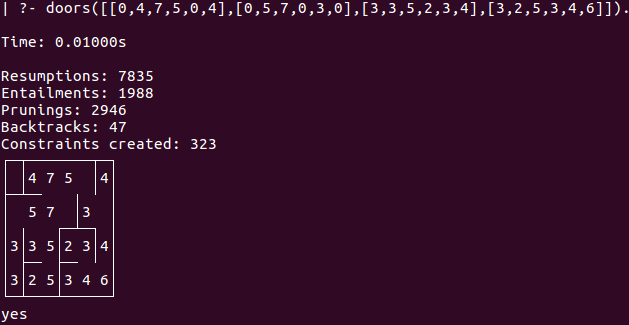
\includegraphics[width=0.8\textwidth]{example1.png}
\caption{Example of a solver execution.}
\label{fig:examples}
\end{figure}

In terms of mere efficiency, on square boards we have the following scores:

\begin{table}[hbtp]
\centering
\begin{tabular}{cccc}
\toprule
number of cells & time   & constraints created & number of backtracks \\
\midrule
9               & 0.00s  & 150                 & 0                    \\
25              & 0.00s  & 626                 & 5                    \\
49              & 0.00s  & 2058                & 146                  \\
64              & 0.030s & 2963                & 813                  \\
100             & 0.610s & 8767                & 18734                \\
110             & 7.10s  & 52149               & 383107               \\
150             & 61.64s & 12891362            & 10509283             \\
\bottomrule\\
\end{tabular}
\caption{Solver execution statistics on various square board sizes}
\label{tab:time}
\end{table}

\section{Conclusions}
\label{sec:conclusions}

We believe our solution is elegant and straightforward, although not terribly efficient. A problem centered around rooms \textsl{seeing} each other has a solution whose logic restraints do not involve more than one room at a time.

To extend the simple solution we included detailed execution statistics and a nice board display on the console.

%
% ---- Bibliography ----
%
% BibTeX users should specify bibliography style 'splncs04'.
% References will then be sorted and formatted in the correct style.
%
% \bibliographystyle{splncs04}
% \bibliography{mybibliography}
%
\begin{thebibliography}{8}
	\bibitem{ref_article1}
	Author, F.: Article title. Journal \textbf{2}(5), 99--110 (2016)
	
	\bibitem{ref_lncs1}
	Author, F., Author, S.: Title of a proceedings paper. In: Editor,
	F., Editor, S. (eds.) CONFERENCE 2016, LNCS, vol. 9999, pp. 1--13.
	Springer, Heidelberg (2016). \doi{10.10007/1234567890}
	
	\bibitem{ref_book1}
	Author, F., Author, S., Author, T.: Book title. 2nd edn. Publisher,
	Location (1999)
	
	\bibitem{ref_proc1}
	Author, A.-B.: Contribution title. In: 9th International Proceedings
	on Proceedings, pp. 1--2. Publisher, Location (2010)
	
	\bibitem{ref_url1}
	LNCS Homepage, \url{http://www.springer.com/lncs}. Last accessed 4
	Oct 2017
\end{thebibliography}

\newpage

\section{Attachments}
\label{sec:attachments}

\subsection{main.pl}

\begin{center}
\begin{minipage}{0.85\textwidth}
\centering\ttfamily
\begin{lstlisting}[language=Prolog]
:- use_module(library(clpfd)).
:- use_module(library(lists)).
:- use_module(library(random)).

:- compile('src/doors.pl').
:- compile('src/matrix.pl').
:- compile('src/lists.pl').
:- compile('src/print.pl').
:- compile('src/statistics.pl').
:- compile('src/random.pl').
:- compile('src/menus.pl').
:- compile('src/test.pl').

re :- compile('main.pl').
doors :- main_menu.
doors(Board) :- doors_calculator(Board).

\end{lstlisting}
\end{minipage}
\end{center}

\subsection{doors.pl}

\begin{center}
\begin{minipage}{0.85\textwidth}
\centering\ttfamily
\begin{lstlisting}[language=Prolog]
doors_calculator(Board) :-
  length(Board, NRows),
  NRows1 is NRows - 1,
  nth1(1, Board, Line),
  length(Line, NCols),
  NCols1 is NCols - 1,
  create_matrix(NRows, NCols1, Vertical),
  create_matrix(NRows1, NCols, Horizontal),
  % Use 1 for door present and 0 for door absent
  flatten(Vertical, VerticalFlat),
  flatten(Horizontal, HorizontalFlat),
  append(VerticalFlat, HorizontalFlat, Vars),
  domain(Vars, 0, 1),
  % Apply restriction on each cell
  (   for(R, 1, NRows),
      param(Board),
      param(Vertical),
      param(Horizontal),
      param(NCols)
  do  ( for(C, 1, NCols),
        param(Board),
        param(Vertical),
        param(Horizontal),
        param(R)
      do restrict_cell(Board, Vertical, Horizontal, [R,C])
      )
  ),
  reset_timer,
  labeling([ffc], Vars),
  print_time,
  fd_statistics,
  print_board(Board, Vertical, Horizontal).

length_list(N, L) :- length(L, N).
create_matrix(R, C, M) :-
  length_list(R, M),
  maplist(length_list(C), M).

calculate_value([], 0).
calculate_value([H|T], V) :-
  calculate_value(T, V1),
  V #= H + H*V1.
  
\end{lstlisting}
\end{minipage}
\end{center}

\begin{center}
\begin{minipage}{0.85\textwidth}
\centering\ttfamily
\begin{lstlisting}[language=Prolog]
/**
 * restrict_cell/4
 * restrict_cell(+Board, +Vertical, +Horizontal, +Cell).
 * Computes the four accumulators on cell [R,C], and bind them
 * to the value of the respective cell in the Board.
 */
restrict_cell(Board, _, _, [R,C]) :-
  matrixnth1([R,C], Board, 0), !.
restrict_cell(Board, Vertical, Horizontal, [R,C]) :-
  matrixnth1([R,C], Board, Value),
  right_total(Vertical, [R,C], Right),
  left_total(Vertical, [R,C], Left),
  top_total(Horizontal, [R,C], Top),
  bot_total(Horizontal, [R,C], Bot),
  Right + Left + Top + Bot + 1 #= Value.
  
\end{lstlisting}
\end{minipage}
\end{center}

\begin{center}
\begin{minipage}{0.85\textwidth}
\centering\ttfamily
\begin{lstlisting}[language=Prolog]
/**
 * right_total/3
 * right_total(+Vertical, +[R,C], -Total).
 * Compute the accumulator function to the right of cell [R,C].
 */
right_total(Vertical, [R,C], Total) :-
  nth1(R, Vertical, L),
  Pop is C - 1,
  popn(Pop, L, Sublist),
  calculate_value(Sublist, Total).
  
\end{lstlisting}
\end{minipage}
\end{center}

\begin{center}
\begin{minipage}{0.85\textwidth}
\centering\ttfamily
\begin{lstlisting}[language=Prolog]
/**
 * left_total/3
 * left_total(+Vertical, +[R,C], -Total).
 * Compute the accumulator function to the left of cell [R,C].
 */
left_total(Vertical, [R,C], Total) :-
  nth1(R, Vertical, L),
  reverse(L, Reversed),
  matrix_length(Vertical, _, V),
  Pop is V - C + 1,
  popn(Pop, Reversed, Sublist),
  calculate_value(Sublist, Total).
  
\end{lstlisting}
\end{minipage}
\end{center}

\begin{center}
\begin{minipage}{0.85\textwidth}
\centering\ttfamily
\begin{lstlisting}[language=Prolog]
/**
 * top_total/3
 * top_total(+Vertical, +[R,C], -Total).
 * Compute the accumulator function upwards of cell [R,C].
 */
top_total(Horizontal, [R,C], Total) :-
  matrix_col(C, Horizontal, L),
  reverse(L, Reversed),
  matrix_length(Horizontal, H, _),
  Pop is H - R + 1,
  popn(Pop, Reversed, Sublist),
  calculate_value(Sublist, Total).
  
\end{lstlisting}
\end{minipage}
\end{center}

\begin{center}
\begin{minipage}{0.85\textwidth}
\centering\ttfamily
\begin{lstlisting}[language=Prolog]
/**
 * bot_total/3
 * bot_total(+Vertical, +[R,C], -Total).
 * Compute the accumulator function downwards of cell [R,C].
 */
bot_total(Horizontal, [R,C], Total) :-
  matrix_col(C, Horizontal, L),
  Pop is R - 1,
  popn(Pop, L, Sublist),
  calculate_value(Sublist, Total).

\end{lstlisting}
\end{minipage}
\end{center}

\subsection{random.pl}

\begin{center}
\begin{minipage}{0.85\textwidth}
\centering\ttfamily
\begin{lstlisting}[language=Prolog]
door_prob(0.3).
novalue_prob(0.2).

/**
 * generate_random_board/2
 * generate_random_board(+[R,C], -Board)
 * generates a random RxC Board
 */
generate_random_board([R,C], Board) :-
  R1 is R - 1,
  C1 is C - 1,
  create_matrix(R, C1, Vertical),
  create_matrix(R1, C, Horizontal),
  door_prob(Prob),
  populate_matrix(Vertical, [R,C1], Prob),
  populate_matrix(Horizontal, [R1,C], Prob),
  create_matrix(R, C, Board),
  generate_values(Board, [R,C], Vertical, Horizontal).
  
\end{lstlisting}
\end{minipage}
\end{center}


\begin{center}
\begin{minipage}{0.85\textwidth}
\centering\ttfamily
\begin{lstlisting}[language=Prolog]
/**
* populate_matrix/3
* populate_matrix(+Matrix, +[NR,NC], +Prob)
* populates a given Matrix (NRxNC) with a probability (0 =< Prob =< 1) of being 0
* and the rest is 1
*/
populate_matrix(Matrix, [NR,NC], Prob) :-
  ( for(R, 1, NR),
    param(Matrix),
    param(Prob),
    param(NC)
  do  ( for(C, 1, NC),
        param(Matrix),
        param(Prob),
        param(R)
        do ( matrixnth1([R,C], Matrix, V),
            (maybe(Prob), !, V is 0; V is 1)
           )
      )
  ).
  
\end{lstlisting}
\end{minipage}
\end{center}


\begin{center}
\begin{minipage}{0.85\textwidth}
\centering\ttfamily
\begin{lstlisting}[language=Prolog]
/**
* generate_values/4
* generate_values(+Board, +[NR,NC], +Vertical, +Horizontal)
* generates the board (NRxNC) cells' value with the given Vertical doors and Horizontal doors
* each cell has a probability of having value 0
*/
generate_values(Board, [NR,NC],  Vertical, Horizontal) :-
  novalue_prob(Prob),
  ( for(R, 1, NR),
    param(Prob),
    param(Board),
    param(Vertical),
    param(Horizontal),
    param(NC)
  do  ( for(C, 1, NC),
        param(Prob),
        param(Board),
        param(Vertical),
        param(Horizontal),
        param(R)
        do (
            (maybe(Prob), !, matrixnth1([R,C], Board, 0), !;
            calculate_value(Board, Vertical, Horizontal, [R,C]))
          )
      )
  ).
  
\end{lstlisting}
\end{minipage}
\end{center}


\begin{center}
\begin{minipage}{0.85\textwidth}
\centering\ttfamily
\begin{lstlisting}[language=Prolog]
/**
* calculate_value/4
* calculate_value(+Board, +Vertical, +Horizontal, +[R,C])
*/
calculate_value(Board, Vertical, Horizontal, [R,C]) :-
  matrixnth1([R,C], Board, Value),
  right_total(Vertical, [R,C], Right),
  left_total(Vertical, [R,C], Left),
  top_total(Horizontal, [R,C], Top),
  bot_total(Horizontal, [R,C], Bot),
  Value is Right + Left + Top + Bot + 1.


\end{lstlisting}
\end{minipage}
\end{center}

\subsection{statistics.pl}

\begin{center}
\begin{minipage}{0.85\textwidth}
\centering\ttfamily
\begin{lstlisting}[language=Prolog]
reset_timer :- statistics(walltime, _).
print_time :-
  statistics(walltime, [_,T]),
  TS is ((T//10)*10)/1000,
  nl, format('Time: ~5fs ~n~n', [TS]).

\end{lstlisting}
\end{minipage}
\end{center}

\subsection{print.pl}

\begin{center}
\begin{minipage}{0.85\textwidth}
\centering\ttfamily
\begin{lstlisting}[language=Prolog]
/**
 * max_width_number/2
 * max_width_number(+Numbers, -Width).
 * Width is the maximum number of digits of any number in Numbers.
 */
max_width_number(Numbers, Width) :-
  flatten(Numbers, Flat),
  map(number_codes, Flat, Codes),
  map(length, Codes, Widths),
  max_member(Width, Widths).

/**
 * center_number/2
 * center_number(+Width, +Num).
 * Left and right padding for writing numbers in board cells.
 */
center_number(Width, Num) :-
  number_codes(Num, NumberCodes),
  length(NumberCodes, L),
  Rest is Width - L,
  LeftL is integer((Rest + 1) / 2),
  RightL is integer(Rest / 2),
  fill_n(LeftL, ' ', LeftSpaces),
  fill_n(RightL, ' ', RightSpaces),
  atom_chars(Left, LeftSpaces),
  atom_chars(Right, RightSpaces),
  write(Left), write(Num), write(Right).
\end{lstlisting}
\end{minipage}
\end{center}
  
\begin{center}
\begin{minipage}{0.85\textwidth}
\centering\ttfamily
\begin{lstlisting}[language=Prolog]
/**
 * write_connector/4
 * write_connector(+Left, +Right, +Up, +Down).
 * Unicode box drawing connection horizontal and vertical dashes between
 * cells in the board.
 */
write_connector(1, 1, 1, 1) :- write(' ').
write_connector(1, 1, 1, 0) :- write('\x2577\').
write_connector(1, 1, 0, 1) :- write('\x2575\').
write_connector(1, 1, 0, 0) :- write('\x2502\').
write_connector(1, 0, 1, 1) :- write('\x2576\').
write_connector(1, 0, 1, 0) :- write('\x250c\').
write_connector(1, 0, 0, 1) :- write('\x2514\').
write_connector(1, 0, 0, 0) :- write('\x251c\').
write_connector(0, 1, 1, 1) :- write('\x2574\').
write_connector(0, 1, 1, 0) :- write('\x2510\').
write_connector(0, 1, 0, 1) :- write('\x2518\').
write_connector(0, 1, 0, 0) :- write('\x2524\').
write_connector(0, 0, 1, 1) :- write('\x2500\').
write_connector(0, 0, 1, 0) :- write('\x252c\').
write_connector(0, 0, 0, 1) :- write('\x2534\').
write_connector(0, 0, 0, 0) :- write('\x253c\').
\end{lstlisting}
\end{minipage}
\end{center}

\begin{center}
\begin{minipage}{0.85\textwidth}
\centering\ttfamily
\begin{lstlisting}[language=Prolog]
/**
 * write_multiple/2
 * write_multiple(+N, +Char).
 * Write Char N times.
 */
write_multiple(N, Char) :-
  fill_n(N, Char, Bars),
  atom_chars(String, Bars),
  write(String).

/**
 * write_top/2
 * write_top(+Width, +Vertical).
 * Top bar of the board. 
 */
write_top(Width, VerticalRow) :-
  write('\x250c\'), write_multiple(Width, '\x2500\'),
  ( foreach(Vert, VerticalRow),
    param(Width)
  do  write_connector(0, 0, 1, Vert),
      write_multiple(Width, '\x2500\')
  ),
  write('\x2510\'), nl.
\end{lstlisting}
\end{minipage}
\end{center}

\begin{center}
\begin{minipage}{0.85\textwidth}
\centering\ttfamily
\begin{lstlisting}[language=Prolog]
/**
 * write_bot/2
 * write_bot(+Width, +Vertical).
 * Bottom bar of the board.
 */
write_bot(Width, VerticalRow) :-
  write('\x2514\'), write_multiple(Width, '\x2500\'),
  ( foreach(Vert, VerticalRow),
    param(Width)
  do  write_connector(0, 0, Vert, 1),
      write_multiple(Width, '\x2500\')
  ),
  write('\x2518\'), nl.
\end{lstlisting}
\end{minipage}
\end{center}

\begin{center}
\begin{minipage}{0.85\textwidth}
\centering\ttfamily
\begin{lstlisting}[language=Prolog]
/**
 * write_number_row/3
 * write_number_row(+Width, +BoardRow, +VerticalRow).
 * Write a number line of the board.
 */
write_number_row(Width, BoardRow, VerticalRow) :-
  BoardRow = [Front|Tail],
  write('\x2502\'),
  (Front = 0 -> write_multiple(Width, ' '); center_number(Width, Front)),
  ( foreach(Num, Tail),
    foreach(Vert, VerticalRow),
    param(Width)
  do  (Vert = 0 -> write('\x2502\'); write(' ')),
      (Num = 0 -> write_multiple(Width, ' '); center_number(Width, Num))
  ),
  write('\x2502\'), nl.
\end{lstlisting}
\end{minipage}
\end{center}
  
\begin{center}
\begin{minipage}{0.85\textwidth}
\centering\ttfamily
\begin{lstlisting}[language=Prolog]
/**
 * write_horz_row/4
 * write_horz_row(+Width, +VerticalUp, +VerticalDown, +HorizontalRow).
 * Write a line in between number lines of the board.
 */
write_horizontals(Width, VerticalUp, VerticalDown, HorizontalRow) :-
  HorizontalRow = [FrontHorz|HorizontalTail],
  write_connector(1, FrontHorz, 0, 0),
  (FrontHorz = 0 -> write_multiple(Width, '\x2500\'); write_multiple(Width, ' ')),
  ( foreach(Horz, HorizontalTail),
    foreach(Up, VerticalUp),
    foreach(Down, VerticalDown),
    fromto(FrontHorz, PreviousHorz, Horz, BackHorz),
    param(Width)
  do  write_connector(PreviousHorz, Horz, Up, Down),
      (Horz = 0 -> write_multiple(Width, '\x2500\'); write_multiple(Width, ' '))
  ),
  write_connector(BackHorz, 1, 0, 0), nl.
\end{lstlisting}
\end{minipage}
\end{center}

\begin{center}
\begin{minipage}{0.85\textwidth}
\centering\ttfamily
\begin{lstlisting}[language=Prolog]
/**
 * print_board/3
 * print_board(+Board, +Vertical, +Horizontal).
 * Entry point for board drawing.
 */
print_board(Board, Vertical, Horizontal) :-
  max_width_number(Board, Width),
  Board = [FrontBoard|BoardTail],
  Vertical = [FrontVertical|VerticalTail],
  append(Upper, [BackVertical], Vertical),
  write_top(Width, FrontVertical),
  write_number_row(Width, FrontBoard, FrontVertical),
  ( foreach(BoardRow, BoardTail),
    foreach(VerticalDown, VerticalTail),
    foreach(HorizontalRow, Horizontal),
    foreach(VerticalUp, Upper),
    param(Width)
  do  write_horizontals(Width, VerticalUp, VerticalDown, HorizontalRow),
      write_number_row(Width, BoardRow, VerticalDown)
  ),
  write_bot(Width, BackVertical).

\end{lstlisting}
\end{minipage}
\end{center}

\end{document}